% Graphical abstract, 13 cm x 5 cm (journal minimum 1328 x 531 pixels, readable at 5 x 13 cm).
% Every number is taken from the manuscript tables (clean test set, 747 images).
\documentclass[border=0pt]{standalone}
\usepackage[T1]{fontenc}
\usepackage{mathptmx}
\usepackage{tikz}
\usetikzlibrary{positioning,arrows.meta,calc}
\definecolor{ink}{HTML}{1F2937}
\definecolor{dataC}{HTML}{E8F1FB}
\definecolor{trainC}{HTML}{EAF6EC}
\definecolor{auditC}{HTML}{FDF0E6}
\definecolor{xaiC}{HTML}{F1ECFA}
\begin{document}
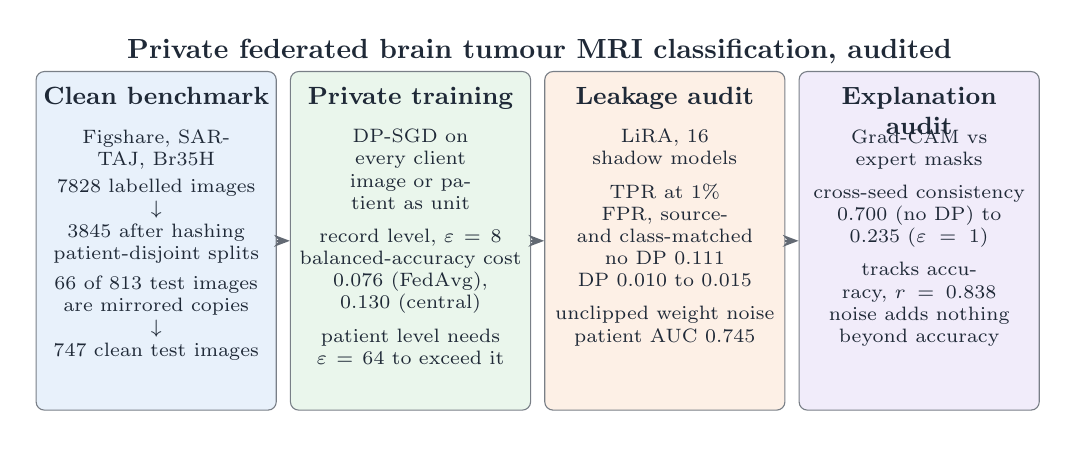
\begin{tikzpicture}[x=1cm,y=1cm, text=ink, >={Stealth[length=2mm]},
  panel/.style={draw=ink!60, rounded corners=3pt, minimum width=3.05cm, minimum height=4.3cm, anchor=north west},
  head/.style={font=\bfseries\small, anchor=north, align=center, text width=2.9cm},
  body/.style={font=\scriptsize, anchor=north, align=center, text width=2.9cm}]
\useasboundingbox (0,0) rectangle (13,5);
\node[font=\bfseries\normalsize, anchor=north] at (6.5,4.98) {Private federated brain tumour MRI classification, audited};
% panel 1
\node[panel, fill=dataC] (p1) at (0.1,4.45) {};
\node[head] at ($(p1.north)+(0,-0.08)$) {Clean benchmark};
\node[body] at ($(p1.north)+(0,-0.62)$) {Figshare, SARTAJ, Br35H\\[2pt]7828 labelled images\\$\downarrow$\\3845 after hashing\\
  patient-disjoint splits\\[3pt]66 of 813 test images\\are mirrored copies\\$\downarrow$\\747 clean test images};
% panel 2
\node[panel, fill=trainC] (p2) at (3.33,4.45) {};
\node[head] at ($(p2.north)+(0,-0.08)$) {Private training};
\node[body] at ($(p2.north)+(0,-0.62)$) {DP-SGD on every client\\image or patient as unit\\[4pt]
  record level, $\varepsilon=8$\\balanced-accuracy cost\\0.076 (FedAvg), 0.130 (central)\\[4pt]
  patient level needs\\$\varepsilon=64$ to exceed it};
% panel 3
\node[panel, fill=auditC] (p3) at (6.56,4.45) {};
\node[head] at ($(p3.north)+(0,-0.08)$) {Leakage audit};
\node[body] at ($(p3.north)+(0,-0.62)$) {LiRA, 16 shadow models\\[4pt]
  TPR at 1\% FPR, source-\\and class-matched\\no DP 0.111\\DP 0.010 to 0.015\\[4pt]
  unclipped weight noise\\patient AUC 0.745};
% panel 4
\node[panel, fill=xaiC] (p4) at (9.79,4.45) {};
\node[head] at ($(p4.north)+(0,-0.08)$) {Explanation audit};
\node[body] at ($(p4.north)+(0,-0.62)$) {Grad-CAM vs expert masks\\[4pt]
  cross-seed consistency\\0.700 (no DP) to 0.235 ($\varepsilon=1$)\\[4pt]
  tracks accuracy, $r=0.838$\\noise adds nothing\\beyond accuracy};
\foreach \a/\b in {p1/p2,p2/p3,p3/p4} \draw[->, draw=ink!70, line width=0.8pt] (\a.east) -- (\b.west);
\end{tikzpicture}
\end{document}
